\documentclass{article}
\usepackage[utf8]{inputenc}
% Si unit
\usepackage{siunitx}
% Set indent 0 for entire document
%\setlength\parindent{0pt}


\title{Ocean optic crash course}
\author{mauhing.yip }
\date{October 2020}

\usepackage{natbib}
\usepackage{graphicx}

\begin{document}

\maketitle

\section{Preface}
This document is meant to give a crash course for AROS member and will only present the knowledge that has been used in our project.

\section{Introduction}
How lights propagate in a clear air medium is well-studied. However, how light propagate in water is a more complicate topic due to scattering and absorption. In this case, many empirical formulas are established from experimental result. Even though the topic is complicate, the knowledge we need for the AROS project is not a lot and understandable. This document will be mostly based on https://oceanopticsbook.info/ but only extract the part we need.

\section{Different optical quantities}
Before we dive into the ocean optic. We need to familiar with different optical quantities. In optical physics, there are two parallel systems used to describe physical properties. The first one is radiometric, and the second one is photometric. The different between them is that the latter taken account for human perception of different color than former. In document, we only care about radiometric quantities and ignore wavelength, which is listed below.

\begin{table}[h]
\centering
\begin{tabular}{|l|l|l|l|}
\hline
\multicolumn{2}{|l|}{Quantity} & Unit                                      & Relation         \\ \hline
Radiant energy    & $Q$        & \si{\joule}                               &                  \\ \hline
Radiant flux      & $\Phi$     & \si{\watt}                                & $dQ/dt$          \\ \hline
Radiant intensity & $I_\omega$ & \si{\watt\per\steradian}                  & $d\Phi/d\omega$  \\ \hline
Radiance          & $L_\omega$ & \si{\watt\per\steradian\per\square\meter} & $dI_\omega/dA$   \\ \hline
Irradiance        & $E$        & \si{\watt\per\square\meter}               & $d\Phi/dA$       \\ \hline
\end{tabular}
\caption{Various optical quantities and relation between them.}
\label{tab:optic}
\end{table}
The subscribe $\omega$ indicate that it is a directional properties. The quantities $\Phi$, $I_\omega$ and $L_\omega$ can both means emission, reflection, transmission and received and depends on wavelength. These are the common physical quantities use in optics, and also ocean optics.
 
\section{K function}
\label{sec:K_func}
Radiances and irradiances all decrease approximately exponentially with depth in homogeneous water when the depth is far enough to be free of boundary effects. Therefore, it is convenient to write the depth dependence of $E_d(z)$, for example, as

\begin{equation}
    E(z) := E(0)\exp[-\int_0^z K(z')dz']
    \label{eq:K}
\end{equation}
where $K_d(z)$ is the diffuse attenuation function. $K$ function should depend strongly on water IOPs (Inherent optical properties). Of course that light will scatter in many direction. But equation \ref{eq:K} describe the how light attenuate in the straight path. Similar equations can be written for other radiometric variables and their corresponding K functions.

In our case, which the $K$ in article \cite{gupta2008controlling} is constant, and denoted as $\sigma$ in their article. 

\section{Volume scattering function}
We also have equation to describe how light scatter in a specific direction when We assume that the light is unpolarized and medium is isotropic. If these two assumptions are true, then the scattering process is azimuthally symmetric:
\begin{equation}
    \beta(\psi) := \lim_{\Delta r \to 0} \lim_{\Delta \Omega \to 0} \frac{\Phi_s(\psi)}{\Phi_i \Delta r \Delta \Omega}
\end{equation}
which $\beta(\psi)$ is called volume scattering function and has unit \si{\per\meter\per\steradian}. Figure \ref{fig:scattering} describe equation \ref{eq:K}. In other words the ratio between outgoing wave to incoming wave is 
\begin{equation}
    \frac{\Phi_s(\psi)}{\Phi_i} \approx \beta(\psi)\Delta r \Delta \Omega.
\end{equation}
Volume scattering function is generally denoted as $\beta$, but we will use $F$ as the symbol as article \cite{gupta2008controlling} does. We will use henyey -greenstein function \cite{Haltrin:02} as our volume scattering function.

\begin{figure}[h]
    \centering
    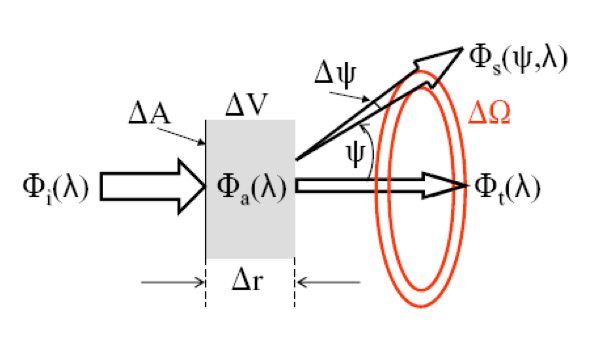
\includegraphics[width=\textwidth]{scattering.png}
    \caption{Volume scattering function. Source: https://oceanopticsbook.info/}
    \label{fig:scattering}
\end{figure}

\section{Albedo}
Albedo is the absorption weight for a give object. An ideally dark material will absorb all the light regardless wavelength. An example is black hole in our universe, and the albedo will be $0$ in this case. An ideally white object will not absorb any light regardless wavelength, it will reflect all light come in. In really, it is always wavelength depends for most of our everyday object. But for simplicity reason, we currently work on only mono-color, we can assume dark surface is close to $0$ and white surface is close to $1$.

\section{Light Transport}
Now, we can use these equations to formulas underwater light transport between camera and light. When a camera looking at the a specific point of an object in the underwater environment while the point is under lighting, there are tree main factors to contribute the a given pixel in the camera. They are direct, indirect and back scattering light transport. Figures \ref{fig:scatter_D}, \ref{fig:scatter_A} and \ref{fig:scatter_B} Here, we discuss them one by one.

\subsection{Direct light transport}
Figures \ref{fig:scatter_D} demonstrate the idea of direct light transport. Light from light source travel directly to object surface and forms diffuse reflection and we assume that the surface is lambertian reflectance, which means the surface has same radiance ($L_\omega$) in all angle. From the equation \ref{eq:K}, the energy of direct light transport is expressed in the following,

\begin{equation}
    D = \frac{I_0}{d_{LO}^2}e^{-\sigma(d_{LO}+d_{CO})}R(\phi),
    \label{eq:D}
\end{equation}
where the $I_0$ is radiant intensity, $d_{LO}$ is the distant between point $L$ and $O$, $R$ is $A \cos\phi$, which is the projection area. In general, $R$ should also include albedo ($albedo$), which it should be $R=\mu A\cos\phi$. But in our case, we factor out $\mu$ and multiply $D$ with $\mu$ later on. Because that is done on the article \cite{gupta2008controlling}. The meaning of $\frac{I_0}{d_{LO}^2}$ is the irradiance on the object surface. It can be proved in the following way. Imaging we have a point light source and it has radiant intensity $I_0$ and an imaginary sphere surface with radius $r$. We denote the irradiance of this sphere as $E$. The relation between $I_0$ and $E$ is the following,
\begin{equation}
    I_0 = \frac{E\cdot4\pi r^2}{4\pi},
\end{equation}
as well as we can see it from table \ref{tab:optic}. Given $I_0$ and $r$, we can calculate $E$ and multiply it with projection area will give us $\Phi$, which meaning energies per second that get received on the surface in vacuum. But light attenuate in underwater, therefore, the factor $e^{-\sigma(d_{LO}+d_{CO})}$ from section \ref{sec:K_func} is introduced.

\begin{figure}[h]
    \centering
    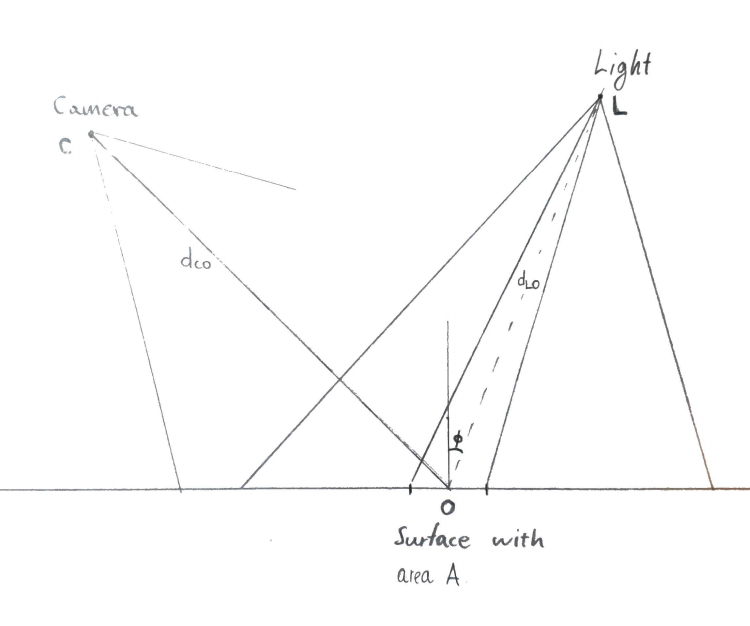
\includegraphics[width=\textwidth]{D.png}
    \caption{Direct light transport}
    \label{fig:scatter_D}
\end{figure}

\subsection{Indirect light transport}
Indirect light transport is combine effect as direct light transport and scattering effect. See figure \ref{fig:scatter_A}. We can image the light travel from $L$ to $X$, and the small volume at $X$ act like a small lamp to scattering light to the object surface. Of course, we need to calculate how much light is scattered to the object surface. The equation for the indirect light transport is in the following,
\begin{equation}
    A =  \int_V \int_\omega \frac{I_0}{d_{LO}^2 d_{XO}^2}e^{-\sigma(d_{LO}+d_{XO}+d_{CO})}R(\gamma)F(\alpha)d\omega dV,
    \label{eq:A}
\end{equation}
where $F$ is our henyey -greenstein function, $d\omega$ is our infinitesimal steradian angle and $dV$ is our infinitesimal volume. We should be not surprise the extra distance factor in the denominator as the infinitesimal volume also act like a light source due to scattering.

\begin{figure}[h]
    \centering
    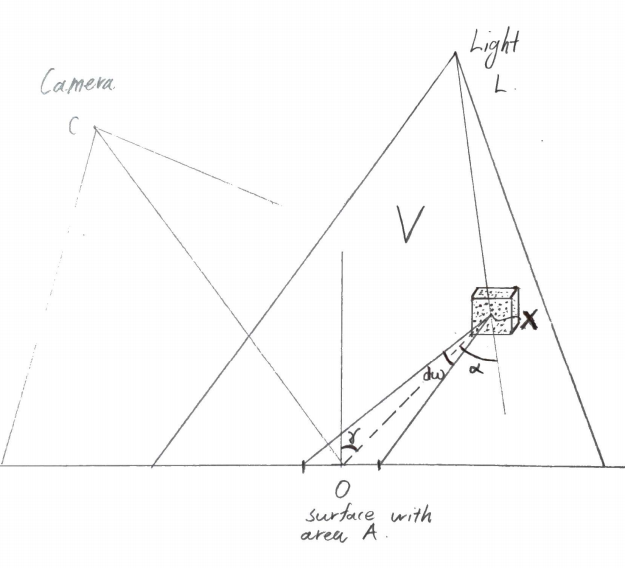
\includegraphics[width=\textwidth]{A.png}
    \caption{Indirect light transport}
    \label{fig:scatter_A}
\end{figure}

\subsection{Back scattering light transport}
The back scattering light transport is similar to indirect light transport, except two things. First one is that we focus on the volume scattering in the path to the object surface. Second one is that we focus on the scattered light from the scattering object, which is shown in figure \ref{fig:scatter_B}. The equation for back scattering is shown in the following:
\begin{equation}
    B =  \int_O^G \int_\omega \frac{I_0}{d_{LY}^2} e^{-\sigma(d_{LY}+d_{YC})}F(\theta)d\omega dY,
    \label{eq:B}
\end{equation}
which $dY$ is the infinitesimal volume. Since the back-scattering destroying image texture, so we want to have light and camera pose to minimize the effect.

\begin{figure}
    \centering
    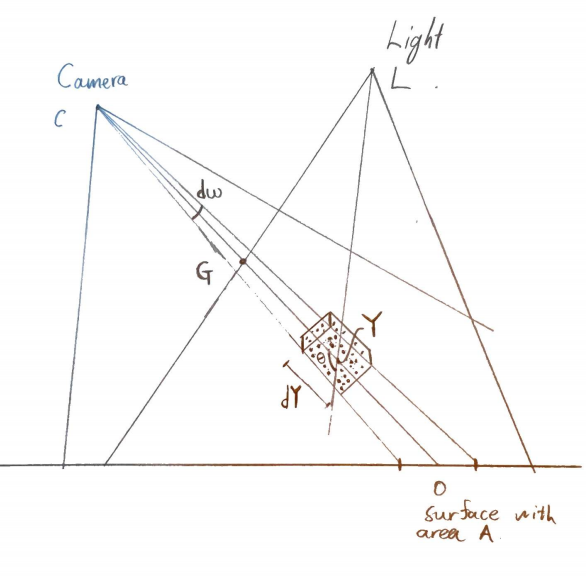
\includegraphics[width=\textwidth]{B.png}
    \caption{Scattering}
    \label{fig:scatter_B}
\end{figure}

\bibliographystyle{plain}
\bibliography{references}
\end{document}
